% gr-Mycielski.tex -- Mycielski's construction : from C5 (triangle-free,
% 3 colours) to the Grotzsch graph (triangle-free, 4 colours).
% u_i : the cycle ; w_i : a shadow of u_i, joined to the neighbours of
% u_i ; z : joined to all the shadows. Engine : pdfLaTeX or LuaLaTeX
\documentclass[border=3mm, convert=false]{standalone}
\usepackage{tkz-berge}
\begin{document}
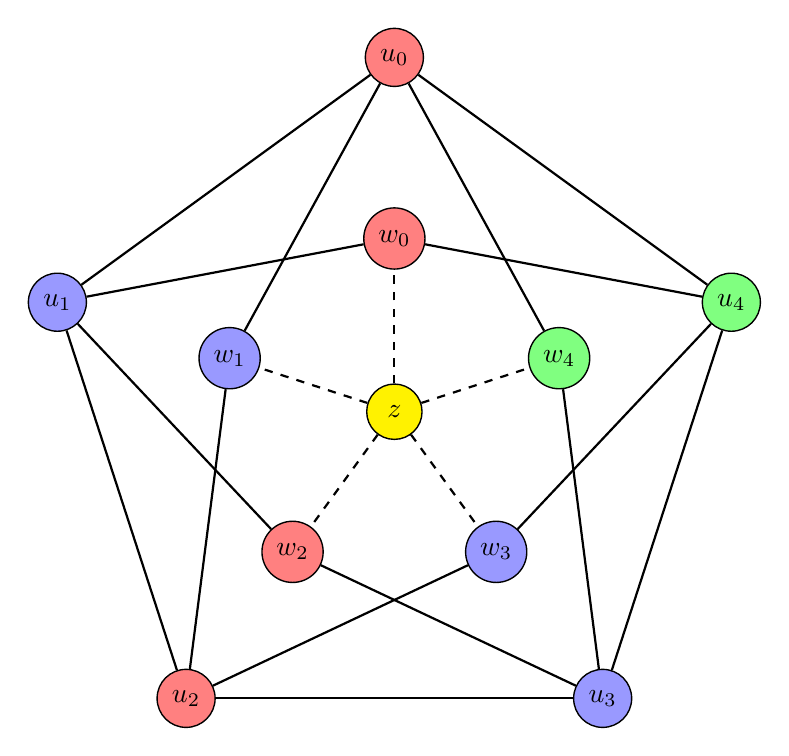
\begin{tikzpicture}
  \GraphInit[vstyle=Normal]
  \SetVertexMath
  \tikzset{VertexStyle/.append style = {minimum size = 20pt}}
  \foreach \i/\c in {0/red!50,1/blue!40,2/red!50,3/blue!40,4/green!50}{%
    \begin{scope}[VertexStyle/.append style = {fill = \c}]
      \Vertex[a=90+72*\i,d=4.5,L={u_{\i}}]{u\i}
      \Vertex[a=90+72*\i,d=2.2,L={w_{\i}}]{w\i}
    \end{scope}}
  \begin{scope}[VertexStyle/.append style = {fill = yellow}]
    \Vertex[x=0,y=0,L=z]{z}
  \end{scope}
  \Edges[lw=1.5pt](u0,u1,u2,u3,u4,u0)
  \foreach \i in {0,...,4}{%
    \pgfmathtruncatemacro\p{mod(\i+4,5)}
    \pgfmathtruncatemacro\n{mod(\i+1,5)}
    \Edge[color=gray](w\i)(u\p)
    \Edge[color=gray](w\i)(u\n)
    \Edge[color=orange,style={dashed}](z)(w\i)}
\end{tikzpicture}
\end{document}
